\chapter{Training, Tuning \& Deployment}\label{ch:training}
\begin{center}\small\textit{Architecture is half the battle -- the rest is making it actually work and stay working in the real world.}\end{center}

\noindent\fbox{\parbox{\dimexpr\linewidth-2\fboxsep-2\fboxrule}{%
\textbf{From zero: no MLOps background assumed.} We start from a model that will not train and build to hyperparameters, debugging checklists, and deployment. Every recipe is motivated by a failure mode first; jargon is defined on first use.}}
\vspace{0.3em}
\section*{Learning Outcomes}
After this chapter you will be able to:
\begin{enumerate}[label=(L\arabic*)]
    \item tune learning rate, batch size, and weight decay on a log scale;
    \item apply a debugging checklist for stalled, diverged, or NaN training;
    \item compare hyperparameter search strategies and ensure reproducibility;
    \item describe deployment concerns: export, monitoring, and MLOps basics.
\end{enumerate}

\section{Intuition: From Toy to Production}
You have a Transformer, a loss, and Adam. Yet training loss stalls, validation diverges, or gradients explode to NaN overnight. Real projects spend 80\% of time on \textbf{hyperparameters, debugging, and deployment} -- not model design. This chapter is the field manual.

\section{Hyperparameters that Matter}
\begin{itemize}
\item \textbf{Learning rate} $\eta$: often the single most important knob. Too high diverges, too low crawls. Search on log scale: $10^{-5}$ to $10^{-1}$. Use LR range test -- increase $\eta$ exponentially for a few epochs, pick the steepest descent before divergence.
\item \textbf{Batch size} $B$: 32--256 typical. Larger $B$ gives stabler gradient but needs larger $\eta$ (linear scaling rule: double $B$, double $\eta$ with warmup). Small $B$ regularizes via noise.
\item \textbf{Weight decay} $\lambda$: $10^{-4}$--$10^{-2}$ for AdamW. Tune jointly with $\eta$.
\item \textbf{Depth/width}: deeper = more capacity but harder to optimize (needs residuals + norm). Wider = more parallelism.
\item \textbf{Regularization}: dropout $0.1$--$0.5$, augmentation strength, label smoothing.
\end{itemize}

\begin{center}
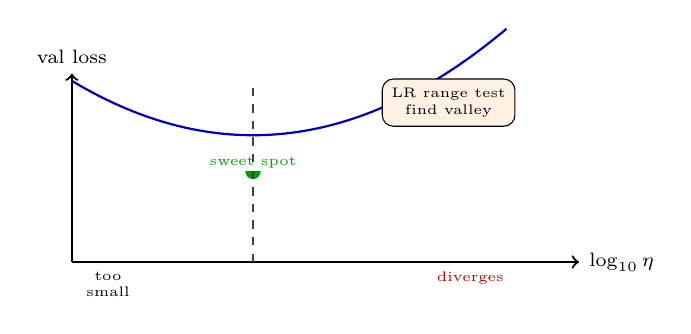
\begin{tikzpicture}[font=\scriptsize, scale=0.92]
  \draw[->, thick] (0,0) -- (7,0) node[right] {$\log_{10}\eta$};
  \draw[->, thick] (0,0) -- (0,2.6) node[above] {val loss};
  \draw[thick, blue!70!black, domain=0:6, samples=80] plot (\x, {2.5-0.6*\x+0.12*\x*\x});
  \fill[green!60!black] (2.5,1.25) circle (3pt) node[above, font=\tiny, fill=white, inner sep=1pt] {sweet spot};
  \node[below, font=\tiny, align=center] at (0.5,0) {too\\small};
  \node[below, font=\tiny, align=center, text=red!70!black] at (5.5,0) {diverges};
  \draw[dashed, gray!50!black] (2.5,0) -- (2.5,2.4);
  \node[draw, fill=orange!10, rounded corners, font=\tiny, align=center] at (5.2,2.2) {LR range test\\find valley};
\end{tikzpicture}
\end{center}

\textbf{Systematic search}: random search beats grid search in high dimensions (Bergstra \& Bengio). For budgets, use \textbf{Bayesian optimization} or \textbf{Hyperband/ASHA} (early-stop bad trials). Always log every run (Weights \& Biases, TensorBoard).

\section{Debugging Checklist}
When loss is NaN or flat, run through this order:

\begin{enumerate}[leftmargin=1.1em]
\item \textbf{Overfit a tiny batch}: train on 8 examples -- if loss does not hit $\approx0$, bug exists (LR too low/high, wrong loss, frozen weights).
\item \textbf{Check data}: visualize augmented images, tokenization, label distribution. Leakage between train/val?
\item \textbf{Gradient norms}: log $\|\nabla\|$ per layer; explosion $\to$ clip; vanishing $\to$ check init/activation/norm.
\item \textbf{Initialization}: Xavier/He. $\text{Var}[W]=2/\text{fan\_in}$ for ReLU (He). Wrong init stalls deep nets.
\item \textbf{Loss scale}: cross-entropy expects logits (no softmax); MSE with unnormalized targets explodes.
\item \textbf{Determinism}: fix seeds, disable nondeterministic cuDNN for reproducibility.
\end{enumerate}

\begin{center}
\begin{tikzpicture}[font=\tiny, >=Stealth, scale=0.90]
  \node[draw, fill=blue!12, rounded corners, minimum width=2.2cm, minimum height=0.8cm, align=center] (a) at (0,0) {Tiny batch\\overfit?};
  \node[draw, fill=green!12, rounded corners, minimum width=2.2cm, minimum height=0.8cm, align=center] (b) at (3.5,0) {Data OK?\\visualize};
  \node[draw, fill=orange!12, rounded corners, minimum width=2.2cm, minimum height=0.8cm, align=center] (c) at (7,0) {Grad/Init\\check};
  \node[draw, fill=violet!12, rounded corners, minimum width=2.2cm, minimum height=0.8cm, align=center] (d) at (10.5,0) {Loss/Scale\\correct?};
  \draw[->, thick, blue!60!black] (a) -- (b);
  \draw[->, thick, blue!60!black] (b) -- (c);
  \draw[->, thick, blue!60!black] (c) -- (d);
  \node[below=0.5cm of b, draw, fill=red!8, rounded corners, align=center, font=\tiny] (fail) {If tiny batch fails\\bug, not data};
  \draw[dashed, red!50!black] (a.south) -- (fail.north);
\end{tikzpicture}
\end{center}

\section{Deployment: Beyond Accuracy}
\begin{itemize}
\item \textbf{Quantization}: FP32 $\to$ INT8 halves memory, speeds 2--4$\times$ on edge. Calibrate ranges; use QAT (quantization-aware training) for $<1\%$ drop.
\item \textbf{Pruning \& distillation}: remove 80\% weights or distill large teacher $\to$ small student via soft targets $p_i^{T}=\text{softmax}(z_i/T)$.
\item \textbf{Latency vs throughput}: batch-1 latency matters for interactive; batch-64 throughput for offline. Profile with TensorRT/ONNX.
\item \textbf{Monitoring}: track input drift (PSI, embedding distance), prediction distribution, and human-evaluated quality. Retrain triggers when drift exceeds threshold.
\item \textbf{Ethics \& safety}: bias audits, adversarial robustness, privacy (DP-SGD), and explainability (SHAP, attention maps).
\end{itemize}

\section{Worked Example: Tuning and Export}
\begin{example}[Hyperparameter Search + ONNX Export]
\begin{lstlisting}[language=Python]
import torch, torch.nn as nn, optuna, onnx
# 1. LR range test
model = nn.Sequential(nn.Linear(64,64), nn.ReLU(), nn.Linear(64,10))
opt = torch.optim.SGD(model.parameters(), lr=1e-7)
lrs, losses = [], []
for lr_mult in [1.2]*100:
    for g in opt.param_groups: g['lr']*=lr_mult
    x,y = next(iter(train_loader))
    loss = nn.CrossEntropyLoss()(model(x), y)
    loss.backward(); opt.step(); opt.zero_grad()
    lrs.append(opt.param_groups[0]['lr']); losses.append(loss.item())

# 2. Optuna search (random/Bayesian)
def objective(trial):
    lr = trial.suggest_float("lr",1e-5,1e-1,log=True)
    wd = trial.suggest_float("wd",1e-6,1e-2,log=True)
    p  = trial.suggest_float("dropout",0.0,0.5)
    # build & train 3 epochs, return val acc
    acc = train_and_eval(lr, wd, p)  # user-defined
    return acc
study = optuna.create_study(direction="maximize")
study.optimize(objective, n_trials=30)
print("Best:", study.best_params)

# 3. Export to ONNX for deployment
dummy = torch.randn(1,64)
torch.onnx.export(model, dummy, "model.onnx", input_names=["input"], output_names=["logits"])
# Quantize / serve with onnxruntime or TensorRT
import onnxruntime as ort
sess = ort.InferenceSession("model.onnx")
print(sess.run(None, {"input": dummy.numpy()})[0].shape)
\end{lstlisting}
\end{example}

Monitoring snippet:
\begin{center}
\begin{lstlisting}[language=Python]
# Drift detection: compare embedding means
import numpy as np
ref_mean = np.load("ref_emb_mean.npy")  # from training
live_emb = model.encode(live_batch)     # current serving
drift = np.linalg.norm(live_emb.mean(0)-ref_mean)
if drift > 0.3:
    print(f"ALERT drift={drift:.2f} -> trigger retrain")
\end{lstlisting}
\end{center}

\section{Putting It All Together}
\begin{center}
\begin{tikzpicture}[font=\scriptsize, >=Stealth, scale=0.88]
  \node[draw, fill=blue!10, rounded corners, minimum width=2.0cm, minimum height=0.8cm, align=center] (a) at (0,0) {Tune\\LR, wd, BS};
  \node[draw, fill=green!10, rounded corners, minimum width=2.0cm, minimum height=0.8cm, align=center] (b) at (3.5,0) {Debug\\tiny batch};
  \node[draw, fill=orange!10, rounded corners, minimum width=2.0cm, minimum height=0.8cm, align=center] (c) at (7,0) {Regularize\\aug, dropout};
  \node[draw, fill=violet!10, rounded corners, minimum width=2.0cm, minimum height=0.8cm, align=center] (d) at (10.5,0) {Deploy\\quant, monitor};
  \draw[->, thick, blue!60!black] (a) -- (b); \draw[->, thick, green!50!black] (b) -- (c); \draw[->, thick, orange!70!black] (c) -- (d);
  \draw[->, thick, violet!60!black, bend left=18] (d) to node[above, font=\tiny] {drift $\to$ retrain} (a);
\end{tikzpicture}
\end{center}

\section{Hyperparameter Search Strategies Compared}
Grid search scales as $k^d$ (exponential in dims) and wastes trials on
irrelevant dims. Random search is embarrassingly parallel and finds good
regions faster (Bergstra \& Bengio, 2012). Bayesian optimization (GP-UCB,
TPE) models $f(\lambda)$ and explores where expected improvement is high --
2--5$\times$ more sample-efficient for expensive training. Hyperband/ASHA
early-stops poor trials, allocating budget to promising ones; combined as
BOHB. Always report search budget and best-vs-final variance.

\section{Initialization and Normalization Deep Dive}
He init assumes ReLU; for GELU/SiLU use $\approx2/\text{fan}_{in}$ as well, but
gain differs. Fixup and T-Fixup initialize deep residual nets without Norm by
scaling residual branches by $L^{-1/2}$. LayerNorm normalizes over features per
token (good for variable length); BatchNorm over batch (good for vision, fails
for small $B$ or sequence). RMSNorm drops mean-centering for speed. Choose
based on modality and batch regime -- mismatching causes instability.

\section{Debugging Case Studies}
Case A: loss flat at init -- check last-layer bias for class imbalance, or
softmax+cross-entropy double-softmax bug. Case B: NaN at step 500 -- usually
FP16 overflow or $\log(0)$; add $\epsilon=10^{-7}$, use BF16, clip logits.
Case C: train acc 95\%, val 60\% -- overfit; add augmentation, dropout, wd,
or more data; check for leakage (duplicates across splits). Case D: val loss
oscillates -- LR too high or batch too small; add warmup, increase $B$, or
use EMA of weights (Polyak averaging) for smoother eval.

\section{Deployment Pipeline and MLOps}
A typical pipeline: train $\to$ validate $\to$ export ONNX $\to$ quantize
(INT8, FP16) $\to$ benchmark (latency, memory, accuracy) $\to$ canary deploy
(5\% traffic) $\to$ monitor (drift, latency P99, error rate) $\to$ rollback
or promote. Use feature stores for consistent train/serve features, and model
registry for versioning. For LLMs, add KV-cache, continuous batching (vLLM),
and speculative decoding for throughput. Cost-aware autoscaling on GPU
utilization keeps spend predictable.

\section{Reproducibility and Ethics Checklist}
Fix all seeds (Python, NumPy, PyTorch, CUDA), set \texttt{CUBLAS\_WORKSPACE\_CONFIG},
and log code+data hashes. Version datasets with DVC. For ethics: measure
subgroup performance (gender, locale), test adversarial robustness (FGSM,
AutoAttack), apply DP-SGD if privacy-sensitive, and document limitations in a
model card. No model is ``done'' at deployment -- it enters a lifecycle of
measurement, mitigation, and update.

\section{Common Pitfalls}
Tuning on test data inflates reported accuracy -- keep test locked. Changing
two hyperparameters at once confounds attribution; use ablations. Not logging
random seeds makes ``improvements'' irreproducible. Overlooking data pipeline
bottlenecks (CPU augmentation, I/O) leaves GPUs idle -- profile with
\texttt{torch.utils.bottleneck}. Finally, optimizing accuracy alone hides
latency/cost: a 0.5\% gain that doubles inference cost may not ship.

\section{Further Reading}
Bergstra \& Bengio (2012) random search; Li et al. (2018) Hyperband; Snoek et
al. Bayesian optimization. For deployment, see Huyen, \emph{Designing ML
Systems}, and PyTorch's quantization guide. For MLOps, explore Weights \&
Biases reports and the ONNX/TensorRT documentation -- the fastest way to cut
latency in practice.

\section{Chapter Summary}
Tuning, debugging, and deployment decide real success. LR $\eta$ matters most
-- find it with range tests and schedules. Tiny-batch overfitting finds bugs
fast; gradient norms, init, and loss scales are the usual suspects. Quantize,
prune, or distill for deployment; monitor drift and canary before full rollout.
Reproducibility (seeds, hashes) and ethics (bias, privacy) are non-optional.

\smallskip
\noindent\textit{Key takeaways:} (1) log-scale search for $\eta,\lambda$;
(2) random $>$ grid; Hyperband prunes early; (3) tiny-batch overfit $=$
smoke test; (4) INT8 + ONNX/TensorRT for serving; (5) drift $>$ threshold
$\to$ retrain.

\section{Exercises}
\begin{exercise} Run an LR range test on a 3-layer MLP on MNIST: sweep $\eta=10^{-6}$ to $10^{-1}$ exponentially for one epoch, plot loss vs $\log\eta$, and pick the optimal $\eta$.\end{exercise}
\begin{exercise} Your loss is NaN after epoch 2. List three likely causes and the log/diagnostic that would reveal each (gradient norm, weight histogram, input stats).\end{exercise}
\begin{exercise} Compare INT8 post-training quantization vs QAT on TinyCNN/CIFAR-10. Report accuracy drop and model size. When does QAT matter most?\end{exercise}
\begin{exercise} Design a Bayesian hyperparameter search space for a Transformer (LR, warmup, wd, dropout, heads). Justify log vs linear scales.\end{exercise}
\begin{exercise} For a production image classifier, propose a monitoring dashboard: three metrics for data drift, three for model health, and a retraining trigger policy.\end{exercise}
% End of Chapter
